\chapter{Determining the coefficient of convective heat transfer}

Date: 20/10/2020

\section{Aim}
The aim of this experiment is to measure the change of temperature of a body as heat flows from it to the surrounding through convective losses where the concept of heat is the flow of thermal energy through conduction, convection, radiation.


\section{Background Theory}
Heat is transferred through conduction, convection and radiation. Conduction is the process whereby heat energy is transferred across a medium. There are materials which are good or poor conductors of heat just like there are materials which are good or bad conductors of electricity. Thus, thermal conduction is the transfer of energy by microscopic collisions of particles and movement of electrons within a body. The equation under thermal equilibrium is as following: 
$$P= \frac{dQ}{dt} = -kA \frac{T_2 - T_1}{L} $$ where P represents power transmitted, A represents area and $T_2 - T_1$ is temperature difference and L represents length. 
Specific heat capacity is defined as amount of energy required per unit mass to raise temperature by one unit. It is given by $$Q=mc \triangle T $$. When heat is lost by object with time then it can be calculated by differentiating the above formula: 
$$\frac{dQ}{dt} = -mc \frac{dT(t)}{dt} $$.

Thermal convection occurs when a liquid comes in contact with an object whose temperature is higher than that of it. When the less energetic molecules of the air encounter the fast vibrating molecules of the hotter object, they pick up some energy off the molecules of the hot surface. At the interface of the object and the air the process is exactly similar to conduction. But the temperature of the air soon rises at the surface causing them to be less dense. The molecules have more energy and the hot air rises. These molecules then transfer the thermal energy to neighboring molecules through collisions conduction as well as through the bulk flow of air convection. In practice, both of these modes of heat transfer go on, hands in hand. When the molecules cool down they become dense and sink and when are hot they become less dense and rise. 

For small temperature difference between a body and its surrounding, the rate of cooling of the body is directly proportional to the temperature difference and the surface area exposed. 

$$\frac{dQ}{dt}  (q – q_s)$$ where q and $q_s$ are temperature corresponding to object and surroundings.

Newton’s law of cooling concerns the process of thermal conduction through convection is mathematically stated as

$$\frac{dQ_{conv}}{dt} = hA(T_2-T_1)$$

When an amount Q heat is provided to cylindrical rod of a certain material to raise its temperature by an amount $\triangle T$. When the rod cools down through convection in air currents the same amount of energy is lost with time to convection. This heat loss is : 
 $$hA(T(t)-T_0) = \frac{dQ}{dt}=-mc \frac{dT(t)}{dt}$$ where T is temperature of rod. $T_0$ is temperature of surrounding, m is mass, A is area of convection and h is coefficient of heat transfer.  


\section{Description of Setup}
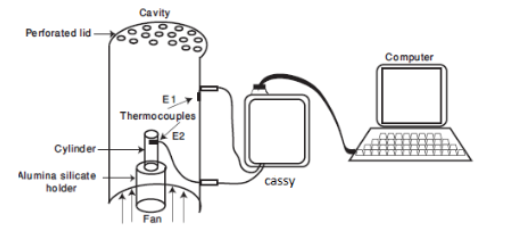
\includegraphics[width=10cm, height=7cm]{figures/fig10.png} \\

The experiment is set up as above where the cylinder is placed inside the cavity to provide a closed environment and a thermocouple is used to measure voltage against the temperature and is inputted into the CASSY software to record readings.Other equipment includes heating machine, graphite powder, weighing machine, temperature gun, and Vernier calipers. 

\section{Method / Procedure}

First the mass is measured using weighing machine, the length and diameter of the cylinders are measured using vernier calipers. Then the cylinder is placed inside the steel box on the hot plate. Then it is covered with graphite powder and heated up to 350 $^{\circ} C$  for 45 minutes.  After heating we attach a thermocouple to the heated cylinder and transfer the cylinder into the cavity with the fan off.One thermocouple is attached to the cylindrical cavity to measure the temperature of the air in the cylinder. Second thermocouple is attached to the heated cylinder through a clip.  Then CASSY software is opened and readings are recorded. The cylinder is removed from the cavity and the thermocouple is attached to another cylinder. Then we transfer the cylinder into the cavity with the fan on. The data is recorded on CASSY software. 

% Highlight the following aspects of the experiment conducted 
% \begin{enumerate}
%     \item What method did you use to perform the experiment?
%     \item What adjustments were made, if any? 
%     \item What data was collected?
%     \item How was it collected?
%     \item Were any calibrations made and what were they?
% \end{enumerate}

% Be precise to, ONLY include scientific background.

\section{Data}
The type B uncertainty in the mass of the rod 1 and rod 2 is $0.000003 grams$ , in the diameter of the rod 1 and rod 2 is $0.000002m$ and in the length of rod 1 and rod 2 is $0.00002m$. 

\begin{center}

\begin{tabular}{|l|l|l|}
\hline
\textbf{}                                               & \textbf{Rod 1} & \textbf{Rod 2} \\ \hline
\textbf{Mass (grams)}                                   & 114.47         & 114.45         \\ \hline
\textbf{Length (mm)}                                    & 24.95          & 25.23          \\ \hline
\textbf{Diameter  (mm)}                                 & 78.53          & 78.42          \\ \hline
\textbf{Specific Heat Capacity of Aluminium (J/(kg*K))} & 887            & 887            \\ \hline
\end{tabular}
\end{center}

\section{Data Analysis}
\begin{equation}
    hA(T(t) - T_0 ) = -mc \frac{dT(t)}{dt}
\end{equation}

\begin{equation}
    hA = \frac{-mc}{T(t) - T_0} \frac{dT(t)}{dt}
\end{equation}

\begin{equation}
   c+ hAt = -mc \times ln (T(t) - T_0)
\end{equation}

\begin{equation}
   c = -mcln (X_0)
\end{equation}

\begin{equation}
    -mcln (X_0)+ hAt = -mc \times ln (X(t))
\end{equation}

\begin{equation}
    -mcln (X_0)+ hAt = -mcln (X(t))
\end{equation}

\begin{equation}
   - hAt = mcln (X(t))  -mcln (X_0)
\end{equation}


\begin{equation}
    X(t) = X_0e^({\frac{-hAt}{mc}})
\end{equation}
\begin{center}
    
Units of h =$ \frac{W}{m^2K} $


\end{center}
\begin{center}
\begin{tabular}{|l|l|l|}
\hline
\textbf{}                                      & \textbf{Rod 1} & \textbf{Rod 2} \\ \hline
\textbf{Mass (grams)}                          & 114.4700       & 114.4500       \\ \hline
\textbf{Mass (kg)}                             & 0.1145         & 0.1145         \\ \hline
\textbf{Length (mm)}                           & 24.9500        & 25.2300        \\ \hline
\textbf{Length (m)}                            & 0.0250         & 0.0252         \\ \hline
\textbf{Diameter  (mm)}                        & 78.5300        & 78.4200        \\ \hline
\textbf{Diameter (m)}                          & 0.0785         & 0.0784         \\ \hline
\textbf{Surface Area }   & 0.0062         & 0.0062         \\ \hline
\end{tabular}
\end{center}

\newpage
\begin{figure}[h!]
    \centering
    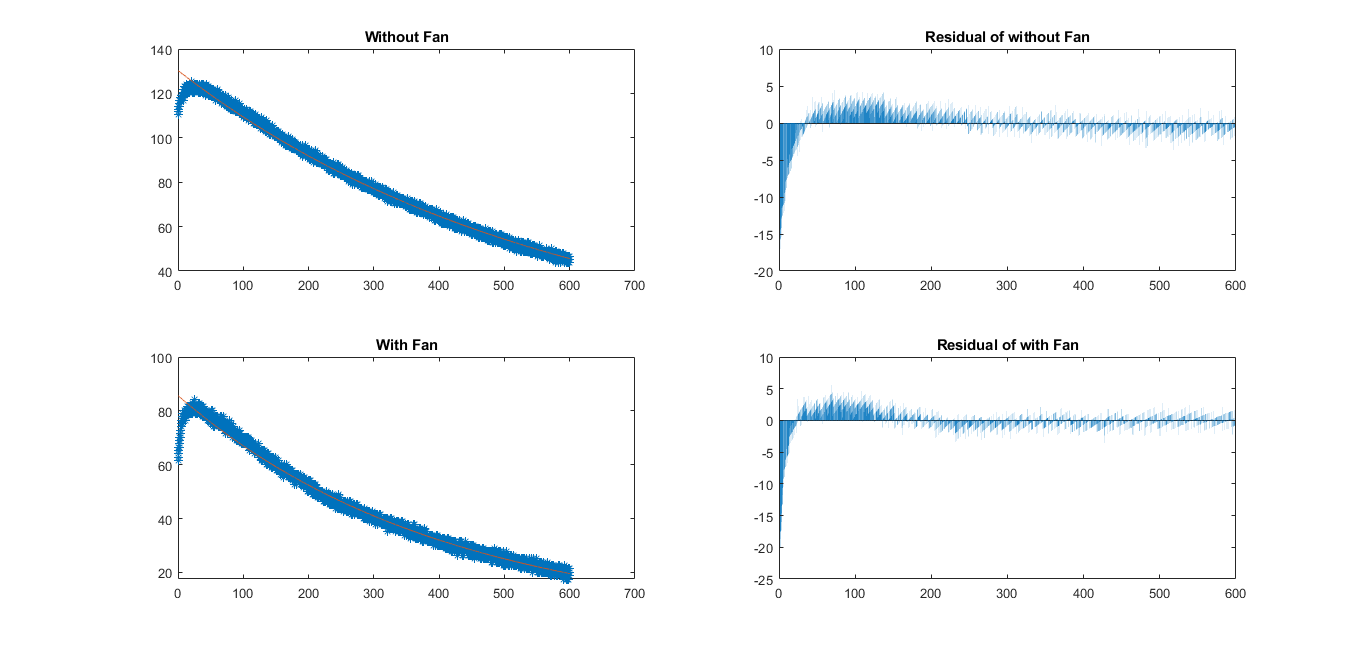
\includegraphics[width=\textwidth]{figures/Subplots.png}
    \caption{Graph of Temperature vs Time}
    \label{fig:yx}
\end{figure}
\begin{center}
    Value of h without fan = $ 28.667 \frac{W}{m^2K} $
\end{center}
\begin{center}
    Value of h with fan = $ 40.1610 \frac{W}{m^2K} $
\end{center}
\section{Discussion \& Conclusion}

As expected as value of h with fan  $ 40.1610 \frac{W}{m^2K} $ is greater than h without fan $ 28.667 \frac{W}{m^2K} $. In the residual graph, there is an irregular pattern which indicates the presence of random error. The major source of this error is the heat loss to the environment. The Newton's Law of cooling is limited because the difference in temperature between the body and surroundings must be small. Another major limitation of Newton’s law of cooling is that the temperature of surroundings must remain constant during the cooling of the body.


\section{MATLAB Script}
\lstinputlisting{matlabCodes/Experiment10.m}



